\documentclass{journal}

\usepackage{multicol}
\usepackage{amsmath}
\usepackage{graphicx}
\usepackage{float}
\usepackage{enumitem}

\title{PID Control of a Robot Via Position Feedback}
\author{Nick Pham}

\begin{document}
%\begin{multicols}{2}

\maketitle

\section*{System Modeling}
The equations of motion for this cart pendulum system are

\begin{align*}
	(m_c + m_p)\ddot{x} + c \dot{x} &= F + m_p r \left( \sin (\theta) \dot{\theta}^2 - \cos (\theta) \ddot{\theta} \right) \\
	\left(J + m_p r^2 \right) \ddot{\theta} + \gamma \dot{\theta} &= -m_p r g \sin (\theta) - m_p r \ddot{x} \cos (\theta)
\end{align*}

which can be linearized to 

\begin{align*}
	(m_c + m_p) \ddot{x} + m_p r \ddot{\theta} + c\dot{x} &= f(t) \\
	m_p r \ddot{x} + \left( J + m_p r^2 \right) \ddot{\theta} + \gamma \dot{\theta} - m_p g r \theta &= 0
\end{align*}

In order to write the state space model, solve for $\ddot{\theta}$ and $\ddot{x}$. Let $M = m_c + m_p$ and $I = J + m_p r^2$.

\begin{align*}
	\ddot{\theta} &= \frac{f(t) - c \dot{x} - M\ddot{x}}{m_p r} \\
	0 &= m_p r \ddot{x} + I \frac{f(t) - c \dot{x} - M\ddot{x}}{m_p r} + \gamma \dot{\theta} - m_p g r \theta \\
	\ddot{x} \left( m_p r - I \frac{M}{m_p r} \right) &= m_p g r \theta - \gamma \dot{\theta} + \frac{Ic \dot{x}}{m_p r} - \frac{I f(t)}{m_p r} \\
	\ddot{x} \left(\frac{m_p^2 r^2 - IM}{m_p r} \right) &= m_p g r \theta - \gamma \dot{\theta} + \frac{Ic \dot{x}}{m_p r} - \frac{I f(t)}{m_p r} \\
\end{align*}

Let $\mu = m_p^2 r^2 - IM$

\begin{align*}
	\ddot{x} \left(\frac{\mu}{m_p r} \right) &= m_p g r \theta - \gamma \dot{\theta} + \frac{Ic \dot{x}}{m_p r} - \frac{I f(t)}{m_p r} \\
	\ddot{x} &= \frac{g}{\mu} \theta - \frac{\gamma m_p r}{\mu} \dot{\theta} + \frac{I}{\mu} (c \dot{x} - f(t))
\end{align*}

Similarly,

\begin{align*}
	\ddot{x} &= \frac{f(t) - c \dot{x} - m_p r \ddot{\theta}}{M} \\
	0 &= m_p r \frac{f(t) - c \dot{x} - m_p r \ddot{\theta}}{M} + I \ddot{\theta} + \gamma \dot{\theta} - m_p g r \theta \\
	\ddot{\theta} \left( I - \frac{m_p^2 r^2}{M} \right) &= m_p g r \theta - \gamma \dot{\theta} + \frac{m_p r}{M} (c\dot{x} - f(t)) \\
	\ddot{\theta} \left( -\frac{\mu}{M} \right) &= m_p g r \theta - \gamma \dot{\theta} + \frac{m_p r}{M} (c\dot{x} - f(t)) \\
	\ddot{\theta} &= - \frac{M}{\mu} m_p g r \theta + \frac{M}{\mu} \gamma \dot{\theta} - \frac{m_p r}{\mu} (c \dot{x} - f(t))
\end{align*}

This means that the state space equations can be written in matrix form

$$
\begin{bmatrix} \dot{x} \\ \dot{\theta} \\ \ddot{x} \\ \ddot{\theta} \end{bmatrix} = \begin{bmatrix} 
	0 & 0 & 1 & 0 \\
	0 & 0 & 0 & 1 \\
	0 & \frac{g}{\mu} & \frac{Ic}{\mu} & - \frac{\gamma m_p r}{\mu} \\
	0 & -\frac{M m_p g r}{\mu} & - \frac{m_p r c}{\mu} & \frac{M \gamma}{\mu}
 \end{bmatrix}
 \begin{bmatrix} x \\ \theta \\ \dot{x} \\ \dot{\theta} \end{bmatrix}
 +
 \begin{bmatrix} 0 \\ 0 \\ -\frac{I}{\mu} \\ - \frac{m_p r}{\mu} \end{bmatrix} f(t)
 $$

Because the system can only observe $x$ and $\theta$, the output is 

$$ \begin{bmatrix} x \\ \theta \end{bmatrix} = \begin{bmatrix} 1 & 1 & 0 & 0 \end{bmatrix} \begin{bmatrix} x \\ \theta \\ \dot{x} \\ \dot{\theta} \end{bmatrix} $$

\section*{Stability Analysis}
Using the A, B, C, D matrices computed in the previous section, simulate the state space model in MATLAB.  Because some of the eigenvalues of $A$ have positive real parts, the system is currently unstable.

The a reasonable step input might be an angle of 0.1.  The resulting step response is shown in Figure \ref{OpenLoopStep}.  As can be seen, the unstable response was indicated by the eigenvalues of $A$.
\begin{figure}
	\centering
	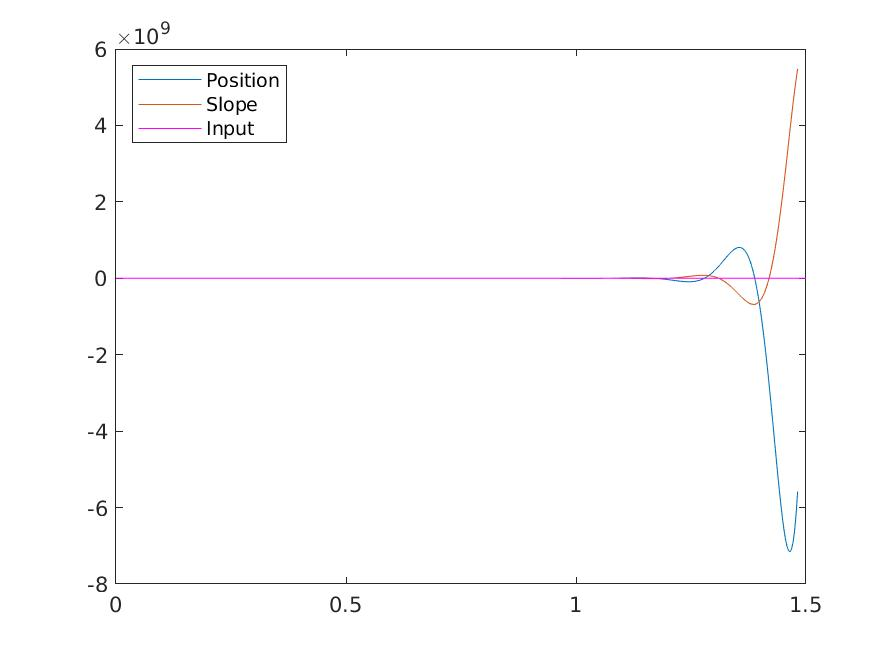
\includegraphics[width = 0.8\textwidth]{ES155Lab2_1b_step}
	\caption{Unstable step response of open loop system.}
	\label{OpenLoopStep}
\end{figure}

\section*{Full State Feedback}
To implement a feedback control system of the form $u = -Kx$, the new state space model would be

\begin{align*}
	\dot{x} &= Ax + Bu = Ax - BKx = (A - BK)x\\
	y &= Cx + Du
\end{align*}

Thus, for a stable system, the eigenvalues of $(A - BK)$ must have negative real parts.  MATLAB's $\mathtt{place()}$ function is used to set $K$ for a given vector of eigenvalues, which can be seen in the attached code.  Figure \ref{ClosedLoopStep} shows the step responses for increasing eigenvalues.  As can be seen, with larger magnitude eigenvalues the system allows less deviation and has quicker stabilization than with smaller eigenvalues.

\begin{figure}
	\centering
	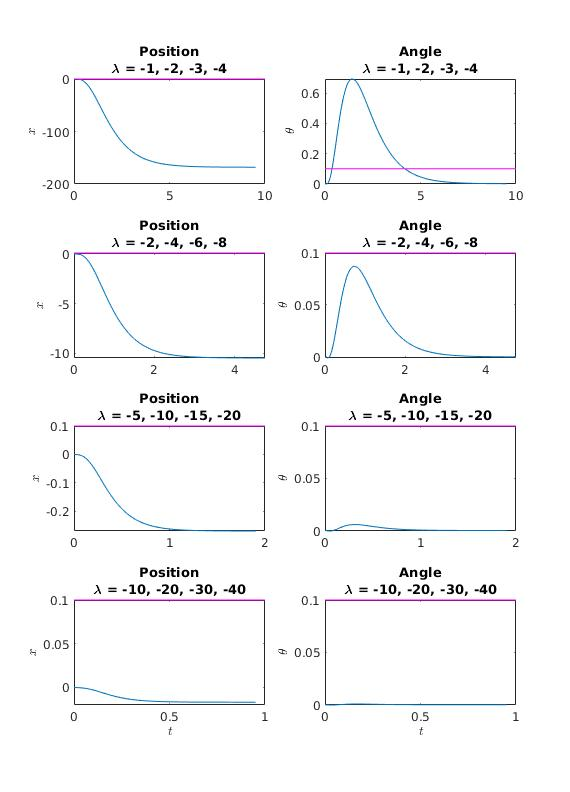
\includegraphics[width = 0.8\textwidth]{ES155Lab2_1c_steps.jpg}
	\caption{Step response of closed loop system with different controllers.}
	\label{ClosedLoopStep}
\end{figure}

\section*{Hardware Implementation}

The system was tested with the following $K$ values, and the system response was observed.

\begin{center}
\begin{tabular}{|c c c c| p{3cm} | p{5cm} |}
	\hline
	$k_p^x$ & $k_d^x$ & $k_p^\theta$ & $k_d^\theta$ & Observation & Explanation \\
	\hline
	20 & 40 & -100 & -20 & Balanced and Smooth & Factory Setting \\
	30 & 40 & -100 & -20 & More Reactive to presses.  Wants to keep $x$ centered but not as resistant to pushes for balancing. & Increasing the importance of the $x$ control in relation to the $\theta$ control means that the angle control will be less effective.\\
	40 & 40 & -100 & -20 & Very jittery, overshoots even without a tap. & The large $x$ proportional control means that the system attempts to correct any errors with a large force, which results in overshoot.  This oscillation prevents the system from converging.\\
	10 & 40 & -100 & -20 & Drifts somewhat in $x$, but quite robust in $\theta$.& Now the tradeoff works the other way, where the effectiveness of the angle control is prioritized.\\
	5  & 40 & -100 &-20 & The pendulum can be pushed in the $x$ axis, while it remains upright despite large forces. & Because there is so little emphasis on the $x$ control, the system only attempts to correct for it when there is no external input.  Otherwise, it works hard to keep the pendulum upright.\\
	20 & 40 & -50 & -20 & Easy to knock over. & This strong deemphasis on the angular control means that the system is easy to tip over.  The gears were also slipping quite a bit, which meant that the angular controller did not have a good mechanism to control the system, contributing to the tipping.\\
	20 & 40 & -150 & -20 & Decent at balancing despite the slipping gears.  Drifts in $x$. & The large proportional angular control allows the system to balance despite physical imperfections.\\
	20 & 40 & -150 & -30 & Jittery behavior reduces convergence. & At this point, the physical system barely worked because of the gears, but increasing the derivative control resulted in a decrease in convergence. \\
	\hline
\end{tabular}
\end{center}

The major takeaways from this lab were the importance in balancing controller parameters in multiple input single output systems, where prioritizing one input results in reduced performance for the other.  Another takeaway was the difficulty of implementing ideal controllers in hardware, where many imperfections are difficult to model.


%\end{multicols}
\end{document}